\documentclass[addpoints]{exam}

\usepackage{verbatim, multicol, tabularx,hyperref, tikz, tikz-qtree, enumitem}
\usepackage{amsmath,amsthm, amssymb, stmaryrd, latexsym, bm, listings}
\usepackage[margin=1in]{geometry}

\usetikzlibrary{shapes}

\lstset{
  extendedchars=\true,
  inputencoding=utf8,
  literate=
  {é}{{\'{e}}}1
  {è}{{\`{e}}}1
  {ê}{{\^{e}}}1
  {ë}{{\¨{e}}}1
  {û}{{\^{u}}}1
  {ù}{{\`{u}}}1
  {â}{{\^{a}}}1
  {à}{{\`{a}}}1
  {î}{{\^{i}}}1
  {ô}{{\^{o}}}1
  {ç}{{\c{c}}}1
  {Ç}{{\c{C}}}1
  {É}{{\'{E}}}1
  {Ê}{{\^{E}}}1
  {À}{{\`{A}}}1
  {Â}{{\^{A}}}1
  {Î}{{\^{I}}}1
  {Ö}{{\"O}}1
  {Ä}{{\"A}}1
  {Ü}{{\"U}}1
  {ö}{{\"o}}1
  {ä}{{\"a}}1
  {ü}{{\"u}}1
  {ß}{{\ss}}1
  ,
  aboveskip=1mm,
  belowskip=1mm,
  showstringspaces=false,
  columns=flexible,
  basicstyle={\scriptsize\ttfamily},
  numbers=left,
  frame=single,
  framextopmargin=0pt,
  framexbottommargin=0pt,
  breaklines=true,
  breakatwhitespace=true,
  keywordstyle=\color{blue},
  identifierstyle=\color{violet},
  stringstyle=\color{teal},
  commentstyle=\color{darkgray}
}

\hypersetup{colorlinks=true,urlcolor=blue}

\headheight = 0.05 in
\headsep = 0.05 in
\parskip = 0.05in
\parindent = 0.0in
\floatsep = 0.05in

\DeclareMathOperator*{\argmin}{arg\!min}
\DeclareMathOperator*{\argmax}{arg\!max}

\title{Adversarial Search Review}
\author{Artificial Intelligence}
\date{}

\begin{document}
\maketitle

\begin{questions}


\setcounter{section}{0} % So that next \section is 1

\question What is a zero-sum game?

\begin{solution}[1in]
\end{solution}

\question What is another,perhaps better, term for zero-sum?  Why?

\begin{solution}[1in]
\end{solution}

\question What is a ply?

\begin{solution}[1in]
\end{solution}

\question In the following 2-ply minimax game tree, what are the minimax values of nodes A, B, C, and D, and which move is selected by MAX?

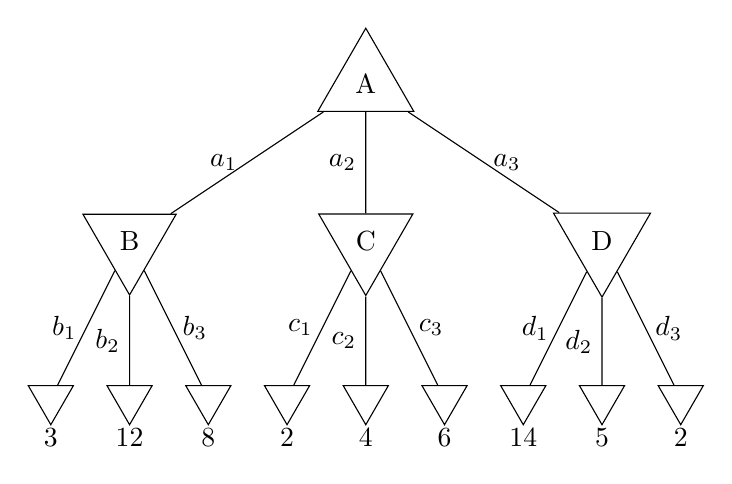
\begin{tikzpicture}[]
  \tikzstyle{max}=[regular polygon,regular polygon sides=3, draw, minimum size=.25cm]
  \tikzstyle{min}=[regular polygon,regular polygon sides=3, draw, shape border rotate=180]

\node[max](A) at (6, 5){A};

\node[min](B) at (3, 3){B};
\node[min](C) at (6, 3){C};
\node[min](D) at (9, 3){D};

\node[min](B1) at (2, 1){};
\node[min](B2) at (3, 1){};
\node[min](B3) at (4, 1){};

\node[min](C1) at (5, 1){};
\node[min](C2) at (6, 1){};
\node[min](C3) at (7, 1){};

\node[min](D1) at (8, 1){};
\node[min](D2) at (9, 1){};
\node[min](D3) at (10, 1){};

\node[](B1val) at (2,0.5){3};
\node[](B2val) at (3,0.5){12};
\node[](B3val) at (4,0.5){8};

\node[](C1val) at (5,0.5){2};
\node[](C2val) at (6,0.5){4};
\node[](C3val) at (7,0.5){6};

\node[](D1val) at (8,0.5){14};
\node[](D2val) at (9,0.5){5};
\node[](D3val) at (10,0.5){2};

\draw (A) to node [left,pos=0.5]{$a_1$} (B);
\draw (A) to node [left,pos=0.5]{$a_2$} (C);
\draw (A) to node [right,pos=0.5]{$a_3$} (D);

\draw (B) to node [left,pos=0.5]{$b_1$} (B1);
\draw (B) to node [left,pos=0.5]{$b_2$} (B2);
\draw (B) to node [right,pos=0.5]{$b_3$} (B3);

\draw (C) to node [left,pos=0.5]{$c_1$} (C1);
\draw (C) to node [left,pos=0.5]{$c_2$} (C2);
\draw (C) to node [right,pos=0.5]{$c_3$} (C3);

\draw (D) to node [left,pos=0.5]{$d_1$} (D1);
\draw (D) to node [left,pos=0.5]{$d_2$} (D2);
\draw (D) to node [right,pos=0.5]{$d_3$} (D3);

\end{tikzpicture}


\begin{solution}[1in]
\end{solution}

\question In the following game tree, what are the $\alpha$ and $\beta$ values in the intervals and which branches would be pruned from the tree with Alpha-Beta pruning?


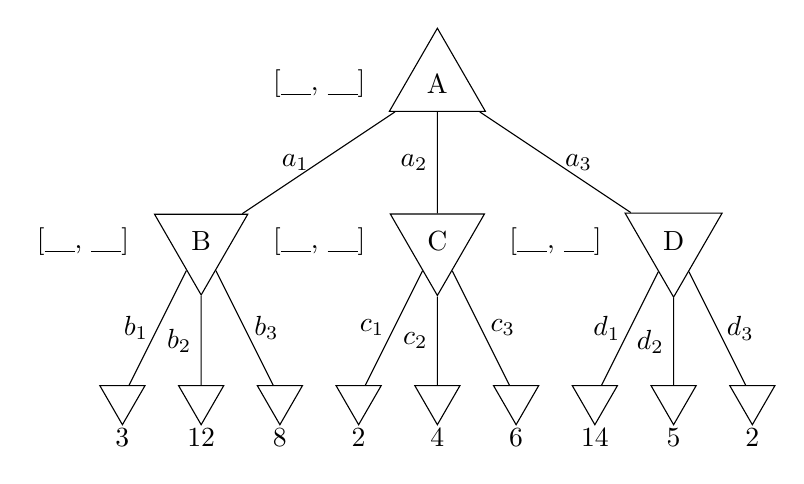
\begin{tikzpicture}[]
  \tikzstyle{max}=[regular polygon,regular polygon sides=3, draw, minimum size=.25cm]
  \tikzstyle{min}=[regular polygon,regular polygon sides=3, draw, shape border rotate=180]

\node[max](A) at (6, 5){A};
\node[] at (4.5, 5){[\underline{\hspace{.15in}}, \underline{\hspace{.15in}}]};

\node[min](B) at (3, 3){B};
\node[] at (1.5, 3){[\underline{\hspace{.15in}}, \underline{\hspace{.15in}}]};

\node[min](C) at (6, 3){C};
\node[] at (4.5, 3){[\underline{\hspace{.15in}}, \underline{\hspace{.15in}}]};

\node[min](D) at (9, 3){D};
\node[] at (7.5, 3){[\underline{\hspace{.15in}}, \underline{\hspace{.15in}}]};

\node[min](B1) at (2, 1){};
\node[min](B2) at (3, 1){};
\node[min](B3) at (4, 1){};

\node[min](C1) at (5, 1){};
\node[min](C2) at (6, 1){};
\node[min](C3) at (7, 1){};

\node[min](D1) at (8, 1){};
\node[min](D2) at (9, 1){};
\node[min](D3) at (10, 1){};

\node[](B1val) at (2,0.5){3};
\node[](B2val) at (3,0.5){12};
\node[](B3val) at (4,0.5){8};

\node[](C1val) at (5,0.5){2};
\node[](C2val) at (6,0.5){4};
\node[](C3val) at (7,0.5){6};

\node[](D1val) at (8,0.5){14};
\node[](D2val) at (9,0.5){5};
\node[](D3val) at (10,0.5){2};

\draw (A) to node [left,pos=0.5]{$a_1$} (B);
\draw (A) to node [left,pos=0.5]{$a_2$} (C);
\draw (A) to node [right,pos=0.5]{$a_3$} (D);

\draw (B) to node [left,pos=0.5]{$b_1$} (B1);
\draw (B) to node [left,pos=0.5]{$b_2$} (B2);
\draw (B) to node [right,pos=0.5]{$b_3$} (B3);

\draw (C) to node [left,pos=0.5]{$c_1$} (C1);
\draw (C) to node [left,pos=0.5]{$c_2$} (C2);
\draw (C) to node [right,pos=0.5]{$c_3$} (C3);

\draw (D) to node [left,pos=0.5]{$d_1$} (D1);
\draw (D) to node [left,pos=0.5]{$d_2$} (D2);
\draw (D) to node [right,pos=0.5]{$d_3$} (D3);

\end{tikzpicture}


\begin{solution}[2.5in]

\end{solution}

\question In basic minimax search, the $Minimax$ value function is defined by:

$$
Minimax(s) =
\begin{cases}
Utility(s,MAX)                              & \text{if } IsTerminal(s) \\
max_{a \in Actions(s)} Minimax(Result(s,a)) & \text{if } ToMove(s) = MAX \\
min_{a \in Actions(s)} Minimax(Result(s,a)) & \text{if } ToMove(s) = MIN
\end{cases}
$$

How does the minimax algorithm and the $minimax$ value function change when using a heuristic static evaluation function?

\begin{solution}[2in]
We add a depth parameter, $d$, which limits the number of plies of the game tree generated by the algorithm, and use this updated $Minimax$ function:

$$
HMinimax(s, d) =
\begin{cases}
Eval(s,MAX)                                        & \text{if } IsCutoff(s, d) \\
max_{a \in Actions(s)} HMinimax(Result(s,a), d+1) & \text{if } ToMove(s) = MAX \\
min_{a \in Actions(s)} HMinimax(Result(s,a), d+1) & \text{if } ToMove(s) = MIN
\end{cases}
$$

\end{solution}

\question In terminal states, what is the value of the $Eval(s, MAX)$ function?

\begin{solution}[1in]
In terminal states, $Eval(state, player) = Utility(state, player)$, which is defined by the game rules.
\end{solution}

\question How does Monte-Carlo Tree Search differ from Heuristic Alph-Beta Search?

\begin{solution}[1.5in]
Instead of searching to a given depth and applying a heurstic evaluation function to the resulting positions, we
\begin{itemize}
\item simulate complete games (from a given position) to terminal positions, and
\item back-up the win/loss scores up the tree.
\end{itemize}
\end{solution}

\question Which weaknesses of Heuristic Alph-Beta Search does MCTS seek to overcome?

\begin{solution}[1.5in]
Two major weaknesses of heuristic alpha-beta tree search:

\begin{itemize}
\item Can't handle high branching factors. Go has a branching factor that starts at 361, which means alpha–beta search would be limited to only 4 or 5 ply.
\item Can't always define a good static evaluation function.  E.g., in Go material value is not a strong indicator and most positions are in flux until the endgame.
\end{itemize}
\end{solution}

\question Using

\begin{solution}[1in]
\end{solution}


\end{questions}

\end{document}
